\documentclass[11pt,letterpaper]{article}

%% ── Packages ──────────────────────────────────────────────────────────────
\usepackage[T1]{fontenc}
\usepackage{lmodern}
\usepackage[margin=1in,top=1.25in]{geometry}
\setlength{\headheight}{22pt}
\addtolength{\topmargin}{-10pt}
\usepackage{graphicx}
\usepackage{hyperref}
\usepackage{xcolor}
\usepackage{listings}
\usepackage{booktabs}
\usepackage{enumitem}
\usepackage{amsmath}
\usepackage{amssymb}
\usepackage{fancyhdr}
\usepackage{titlesec}
\usepackage{longtable}
\usepackage{array}
\usepackage{tabularx}
\usepackage{colortbl}
\usepackage{parskip}
\usepackage{microtype}
\usepackage{hyphenat}
\setlength{\emergencystretch}{3em}
\usepackage{needspace}
\usepackage[right,running]{lineno}
\usepackage{subcaption}

%% ── Suppress lineno inside code listings ────────────────────────────────
\makeatletter
\let\cgns@orig@lstlisting\lstlisting
\let\cgns@endorig@lstlisting\endlstlisting
\renewenvironment{lstlisting}
  {\par\needspace{5\baselineskip}\nolinenumbers\cgns@orig@lstlisting}
  {\cgns@endorig@lstlisting\par\linenumbers}
\makeatother

%% ── Color palette ───────────────────────────────────────────────────────
\definecolor{cgnsblue}{HTML}{1F4E79}
\definecolor{cgnsteal}{HTML}{2E7D8C}
\definecolor{cgnslight}{HTML}{D6EAF0}
\definecolor{cgnsgold}{HTML}{C78C1C}

%% ── Hyperlink style ──────────────────────────────────────────────────────
\hypersetup{
  colorlinks=true,
  linkcolor=cgnsblue,
  urlcolor=cgnsteal,
  citecolor=cgnsblue,
}

%% ── Code listing style ──────────────────────────────────────────────────
\lstset{
  basicstyle=\scriptsize\ttfamily,
  keywordstyle=\bfseries\color{cgnsblue},
  commentstyle=\itshape\color{cgnsteal},
  stringstyle=\color{red!60!black},
  breaklines=true,
  frame=single,
  framerule=0.5pt,
  rulecolor=\color{cgnsblue!40},
  backgroundcolor=\color{cgnslight!30},
  numbers=left,
  numberstyle=\tiny\color{cgnsblue!50},
  numbersep=6pt,
  showstringspaces=false,
  xleftmargin=1em,
  xrightmargin=1em,
  aboveskip=1em,
  belowskip=1em,
  tabsize=4,
}

%% ── SIDS-style node definition environment ──────────────────────────────
\newenvironment{sidsnode}[1]{%
  \par\vspace{0.8em}%
  \noindent\colorbox{cgnslight!50}{\makebox[\dimexpr\linewidth-2\fboxsep][l]{%
    \texttt{\textbf{\color{cgnsblue}#1}}}}\\[0.3em]%
  \begin{quote}\ttfamily
}{%
  \end{quote}\vspace{0.4em}%
}

%% ── Math convenience macros ─────────────────────────────────────────────
\newcommand{\Lsp}{\mathcal{L}_p}
\newcommand{\Qtp}{\mathcal{Q}^{2}_p}
\newcommand{\Qthp}{\mathcal{Q}^{3}_p}
\newcommand{\Ptp}{\mathcal{P}^{2}_p}
\newcommand{\Pthp}{\mathcal{P}^{3}_p}
\newcommand{\Vpq}{\mathcal{V}_{p,q}}

%% ── Header / Footer ────────────────────────────────────────────────────
\pagestyle{fancy}
\fancyhf{}
\fancyhead[L]{\small\color{cgnsblue} CPEX~0045 --- High-Order Polynomial Interpolation}
\fancyhead[R]{\small\color{cgnsblue} Version 2.0}
\fancyfoot[C]{\small\color{cgnsblue}\thepage}
\renewcommand{\headrulewidth}{0.5pt}
\renewcommand{\headrule}{\hbox to\headwidth{\color{cgnsgold}\leaders\hrule height\headrulewidth\hfill}}
\renewcommand{\footrulewidth}{0pt}

%% ── Title Formatting ───────────────────────────────────────────────────
\titleformat{\section}{\Large\bfseries\color{cgnsblue}}{\thesection}{0.6em}{}[\vspace{0.2em}{\color{cgnsgold}\titlerule[0.8pt]}]
\titleformat{\subsection}{\large\bfseries\color{cgnsblue!85}}{\thesubsection}{0.6em}{}
\titleformat{\subsubsection}{\normalsize\bfseries\color{cgnsteal}}{\thesubsubsection}{0.6em}{}

%% =====================================================================
\begin{document}
\linenumbers

%% ── Title Block ─────────────────────────────────────────────────────────
\begin{center}
  
\includegraphics[width=0.25\textwidth]{CGNS_logo_1.png}\\[1.2em]
  {\LARGE\bfseries\color{cgnsblue} CGNS Proposal for Extension 0045}\\[0.6em]
  {\Large\color{cgnsteal} Storing Cell-Wise Polynomial Data and Generalising\\
   the Description of Curved Grid Elements}\\[0.4em]
  {\color{cgnsgold}\rule{0.4\textwidth}{0.8pt}}\\[0.6em]
  {\large Version 2.0}\\[0.6em]
  \today
\end{center}

\vspace{1em}

%% ── Metadata Table ──────────────────────────────────────────────────────
\noindent
\rowcolors{2}{cgnslight!30}{white}
\begin{tabular}{@{} >{\bfseries\color{cgnsblue}}l l @{}}
\toprule
CPEX\#            & 0045 \\
Scope             & High-order polynomial interpolation for elements and solutions \\
Champion          & Koen Hillewaert \\
Organization      & Cenaero \\
E-mail            & \href{mailto:koen.hillewaert@cenaero.be}{koen.hillewaert@cenaero.be} \\
Date First Posted & Mar.\ 26, 2019 \\
Date of Revision  & Jun.\ 25, 2019 \\
SIDS Status       & accepted; implementation complete (v4.5.2) \\
Filemap Status    & accepted; implementation complete (v4.5.2) \\
MLL Status        & accepted; implementation complete (v4.5.2) \\
\bottomrule
\end{tabular}

\vspace{1.5em}

\tableofcontents
\newpage

%% ═════════════════════════════════════════════════════════════════════════
\section{Motivation and Scope}
%% ═════════════════════════════════════════════════════════════════════════

The aim is to cater for the large diversity of high-order methods by including a specification of
the interpolation spaces for solutions in the file, fixing the bare essentials: the coordinate
system.  The choice of Lagrangian interpolation spaces is applicable to the mesh as well as the
solution description.  This generalisation will:

\begin{itemize}[leftmargin=2em]
  \item allow accurate representation of data in a range of popular interpolation spaces which
    could otherwise only be approximated;
  \item allow use of the native storage of the application for the Lagrangian description, leading
    furthermore to
    \begin{itemize}
      \item a simpler, more robust, and generic implementation of drivers;
      \item more efficient I/O by straightforwardly dumping data blocks;
      \item avoiding loss of precision for very specific point distributions;
    \end{itemize}
  \item avoid the need to redefine the format for each new interpolation type/order;
  \item cater for space-time methods as well as for ALE computations by including time in the
    functional expressions.
\end{itemize}

Currently it is assumed that high-order intra-element interpolation is \emph{restricted to
unstructured mesh computations}, as structured meshes do not offer the possibility to
individually list elements per order and moreover do not support curved elements.  Both modal and
nodal interpolations are supported.

There is clear potential for future extension via an explicit specification of mathematical
expressions of the individual interpolation functions.  This will increase the flexibility for
modal interpolation approaches.


%% ═════════════════════════════════════════════════════════════════════════
\section{Rationale}
%% ═════════════════════════════════════════════════════════════════════════

This proposal lifts the limitation of fixing the interpolation functions implicitly by imposing
the position of Lagrange control points as proposed for geometric interpolation/curved elements in
CPEX~0036 and CPEX~0038.  Instead, the description of the functional space and its interpolant is
integrated as metadata in the CGNS file in order to allow high flexibility as to the choice of
interpolants or even coordinates, an automatic procedure to allow for very high interpolation
order, and time-dependent interpolants.


%% ═════════════════════════════════════════════════════════════════════════
\section{Extension of the SIDS}
%% ═════════════════════════════════════════════════════════════════════════

\subsection{Conventions}

\textbf{Modifications to the SIDS:}
\begin{itemize}
  \item addition of a new section~3.4: \emph{High-order interpolation}.
\end{itemize}

In the remainder of this section we introduce the different paragraphs (with numbering to be
adapted) that should be added to the new section.

\begin{quote}
``The CGNS standard allows the user to specify their own interpolation approach for both elements
and solution.  The basic principles are:
\begin{enumerate}
  \item The element coordinate system per element type is a fixed convention.
  \item For the solution interpolation per each element type and interpolation order, a separate
    interpolation block is added which provides one of three choices:
    \begin{itemize}
      \item the set of control points for Lagrange interpolants;
      \item the maximum degree of a Pascal polynomial space defined in parametric coordinates;
      \item the maximum degree of a Pascal polynomial space defined in Cartesian
        (non-parametric) coordinates.
    \end{itemize}
    The first two cover parametric interpolation, whereas the last covers
    modal/Cartesian interpolation.
  \item The mesh is always defined using interpolations in parametric space, by specifying the
    set of control points.  The standard will only allow element types defined up to now, in
    order not to modify the element connectivity description.
  \item The interpolation is \emph{not} supposed to be the same for the geometry as for the
    solution, unless explicitly specified that way.
  \item In addition to the spatial coordinates, time can also be used as an independent variable.
\end{enumerate}
The following sections describe how interpolations are specified.''
\end{quote}

% ─────────────────────────────────────────────────────────────────────────
\subsubsection{Interpolation Type Enumeration: \texttt{InterpolationType\_t}}
\label{sec:interpolation-type}
% ─────────────────────────────────────────────────────────────────────────

\begin{quote}
``\texttt{InterpolationType\_t} specifies how the high-order interpolants for the solution are
defined.  \texttt{InterpolationType\_t} can take four values:

\begin{itemize}
  \item \textbf{\texttt{ParametricLagrange}} corresponds to a Lagrange interpolation based upon a
    set of specified control point coordinates in parametric space for a standard interpolation
    space.
  \item \textbf{\texttt{ParametricMonomialsPascal}} corresponds to modal interpolation functions
    in parametric coordinates, based on monomials according to the classical Pascal sets.
  \item \textbf{\texttt{CartesianMonomialsPascal}} corresponds to modal interpolation functions
    in a Cartesian coordinate system, centred on the element and parallel to the main axes.  The
    interpolation functions are based on monomials according to the classical Pascal sets.
  \item \textbf{\texttt{IsoParametric}} corresponds to using the same interpolation functions for
    the solution as for the mesh.''
\end{itemize}
\end{quote}

% ─────────────────────────────────────────────────────────────────────────
\subsection{High-Order Parametric Interpolation}
\label{sec:parametric}
% ─────────────────────────────────────────────────────────────────────────

\begin{quote}
``\textbf{Scope}: The parametric interpolation conventions can be used for specifying both curved
elements (thereby superseding the standard conventions) and the solution.''
\end{quote}

% ─────────────────────────────────────────────────────────────────────────
\subsubsection{Standard Coordinate Systems for Parametric Interpolation}
\label{sec:coord-systems}
% ─────────────────────────────────────────────────────────────────────────

\begin{quote}
``The parametric coordinate system is defined per element following Figure~\ref{fig:coord-systems}.

For space-time computations the coordinate system is extended with one dimension, by the tensor
product of the spatial coordinate system with the parameter interval $[-1,1]$ in parametric time
$\tau$.  The latter corresponds to the physical time slab $[T_n, T_{n+1}]$.''
\end{quote}

\begin{figure}[htbp]
  \centering
  \begin{subfigure}[b]{0.15\textwidth}
    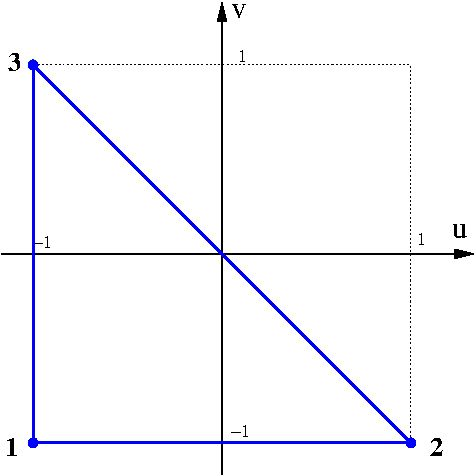
\includegraphics[width=\textwidth]{figures/coord-bar.jpg}
    \caption{BAR}
  \end{subfigure}\hfill
  \begin{subfigure}[b]{0.15\textwidth}
    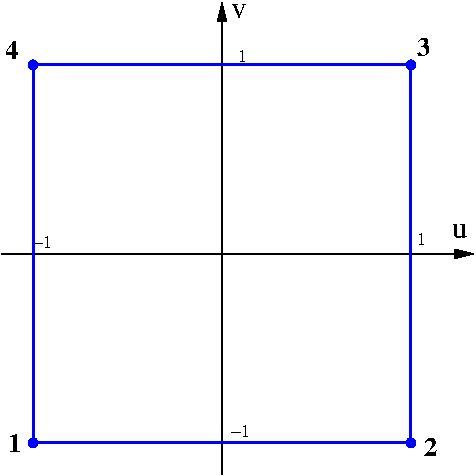
\includegraphics[width=\textwidth]{figures/coord-quad.jpg}
    \caption{QUAD}
  \end{subfigure}\hfill
  \begin{subfigure}[b]{0.25\textwidth}
    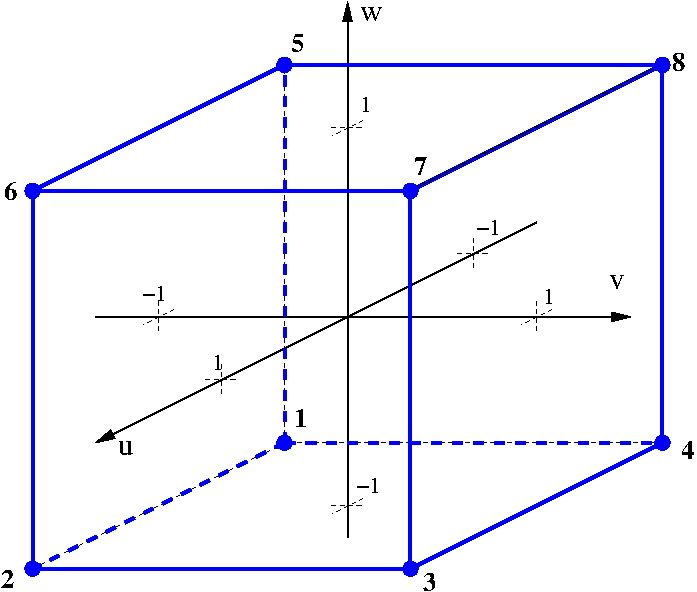
\includegraphics[width=\textwidth]{figures/coord-hexa.jpg}
    \caption{HEXA}
  \end{subfigure}\hfill
  \begin{subfigure}[b]{0.15\textwidth}
    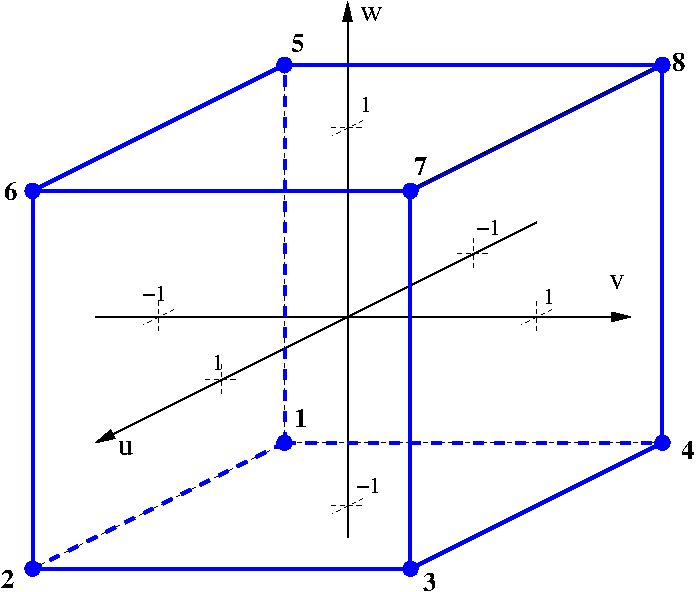
\includegraphics[width=\textwidth]{figures/coord-tri.jpg}
    \caption{TRI}
  \end{subfigure}\hfill
  \begin{subfigure}[b]{0.25\textwidth}
    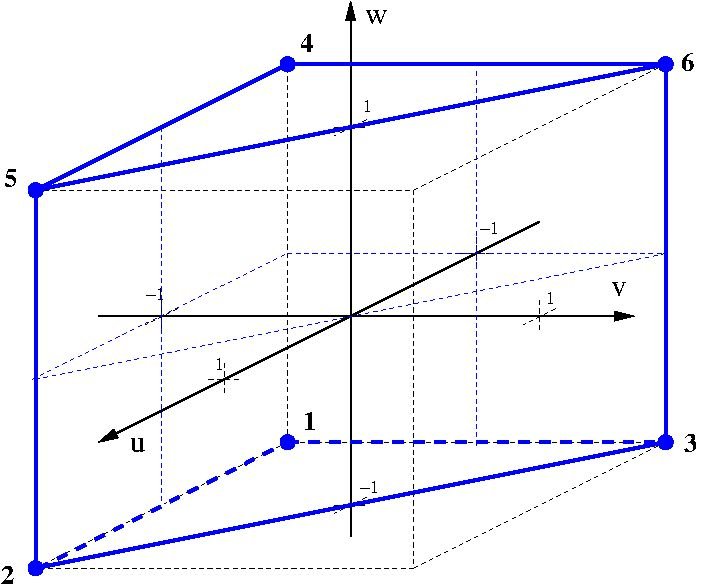
\includegraphics[width=\textwidth]{figures/coord-tetra.jpg}
    \caption{TETRA}
  \end{subfigure}
  \par\vspace{0.5em}
  \begin{subfigure}[b]{0.30\textwidth}
    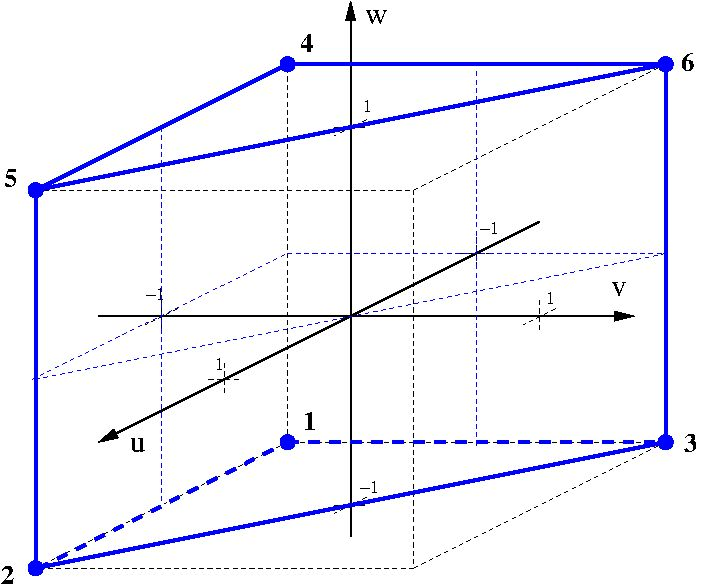
\includegraphics[width=\textwidth]{figures/coord-penta.jpg}
    \caption{PENTA}
  \end{subfigure}
  \caption{Parametric coordinate systems per element type.}
  \label{fig:coord-systems}
\end{figure}

% ─────────────────────────────────────────────────────────────────────────
\subsubsection{Parametric Interpolation by Specification of Lagrange Control Points}
\label{sec:lagrange}
% ─────────────────────────────────────────────────────────────────────────

\begin{quote}
``\textbf{Scope}: Both solution and element shape can be specified using this formulation.  For
elements, this convention allows redefinition of the position and order of the control points with
respect to the standard definitions for each \texttt{ElementType\_t} described in section~3.3.
The standard definition continues to be used when no interpolation is explicitly introduced.

Lagrange interpolants require, next to the specification of control point locations, also the
specification of the standard function space $\mathcal{V}$.  Its cardinality $N$ defines the
number of control points that need to be specified.

We denote the Lagrange interpolant corresponding to control point $\mathbf{u}_i$ as
$\lambda_i$.  Furthermore, we need an arbitrary set of base functions for $\mathcal{V}$, such
that $\mathcal{V} = \mathrm{span}(\psi_j,\; j = 0\ldots N-1)$.  The Lagrange interpolants are
then found as a linear combination of the base functions
%
\begin{equation}
  \lambda_i(\mathbf{u}) = \sum_j V^{-1}_{ij}\, \psi_j(\mathbf{u})
\end{equation}
%
using the inverse of the Vandermonde matrix $V$ associated to the control points $\mathbf{u}_i$
and the basis $\psi$,
%
\begin{equation}
  V_{ij} = \psi_j(\mathbf{u}_i).
\end{equation}

The (spatial) parametric function spaces $\mathcal{V}_p(u,v,w)$ for each element type and order
$p$, which support the Lagrange-type interpolation, are listed in Table~\ref{tab:spaces}.  Next
to the standard ``complete'' element, also incomplete, or so-called serendipity elements are
supported in higher dimensions.  A first type of serendipity element only specifies control
points on the edges.  In three-dimensional elements of sufficient order, a second serendipity
interpolation can be defined which only excludes control points internal to the element.''
\end{quote}

\begin{table}[htbp]
\centering
\caption{Lagrange functional spaces per element and interpolation type.$^{1}$  The base type and
  order $p$ are specified for solution interpolation; the full element type is used to classify
  element interpolation.}
\label{tab:spaces}
\footnotesize
\rowcolors{2}{cgnslight!20}{white}
\begin{tabular}{@{} >{\raggedright\arraybackslash}p{0.09\linewidth}
                    >{\raggedright\arraybackslash}p{0.10\linewidth}
                    >{\raggedright\arraybackslash}p{0.20\linewidth}
                    >{\raggedright\arraybackslash}p{0.40\linewidth}
                    >{\raggedright\arraybackslash}p{0.09\linewidth} @{}}
\toprule
\textbf{Element} & \textbf{Base type} &
  \textbf{Complete} &
  \textbf{Edge Serendipity} &
  \textbf{Face Serendipity} \\
\midrule
Line    & \texttt{BAR\_2}   & $\Lsp(u)$, $N=p+1$
                             & n/a & n/a \\
Quad    & \texttt{QUAD\_4}  & $\Qtp(u,v)$, $N=(p+1)^2$
                             & $\Lsp(u)\otimes\mathcal{L}_1(v) \oplus \Lsp(v)\otimes\mathcal{L}_1(u)$, $N=4p$
                             & n/a \\
Hexa    & \texttt{HEXA\_8}  & $\Qthp(u,v,w)$, $N=(p+1)^3$
                             & & \\
Triangle & \texttt{TRI\_3}  & $\Ptp(u,v)$, $N=\frac{(p+1)(p+2)}{2}$
                             & & n/a \\
Tetra   & \texttt{TETRA\_4} & $\Pthp(u,v,w)$, $N=\frac{(p+1)(p+2)(p+3)}{6}$
                             & & \\
Prism   & \texttt{PENTA\_6} & $\Ptp(u,v)\otimes\Lsp(w)$, $N=\frac{(p+1)^2(p+2)}{2}$
                             & & \\
Pyramid & \texttt{PYRA\_5}  & see~\cite{BCD10} & & \\
\bottomrule
\end{tabular}
\end{table}

{\footnotesize $^{1}$Although for 2D and 3D spaces multi-indices are more convenient, we use
for simplicity of notation a single compounded index $i=(i,j,k)$. Likewise a compound
coordinate $\mathbf{u}=(u,v,w)$ is used.}

\noindent The standard spaces used above are:

\begin{itemize}
  \item The linear space: $\Lsp(u) = \mathrm{span}\{u^i,\; 0 \le i \le p\}$

  \item Tensor product spaces, $N = (p+1)^d$:
  \begin{align*}
    \Qtp(u,v)      &= \Lsp(u) \otimes \Lsp(v)      = \mathrm{span}\{u^i v^j,\; 0 \le i,j \le p\} \\
    \Qthp(u,v,w)   &= \Lsp(u) \otimes \Lsp(v) \otimes \Lsp(w)
                    = \mathrm{span}\{u^i v^j w^k,\; 0 \le i,j,k \le p\}
  \end{align*}

  \item Pascal triangle/tetrahedron, $N = \frac{(p+1)\cdots(p+d)}{d!}$:
  \begin{align*}
    \Ptp(u,v)      &= \mathrm{span}\{u^i v^j,\; 0 \le i+j \le p\} \\
    \Pthp(u,v,w)   &= \mathrm{span}\{u^i v^j w^k,\; 0 \le i+j+k \le p\}
  \end{align*}
\end{itemize}

For space-time function spaces (e.g.\ ALE meshes), the complete functional space is given by
%
\begin{equation}
  \Vpq(u,v,w,t) = \mathcal{V}_p(u,v,w) \otimes \mathcal{L}_q(t)
\end{equation}
%
where $p$ and $q$ are the spatial and temporal orders respectively.

% ─────────────────────────────────────────────────────────────────────────
\subsubsection{Parametric Modal Interpolation}
\label{sec:parametric-modal}
% ─────────────────────────────────────────────────────────────────────────

\begin{quote}
``\textbf{Scope}: This type of interpolation only applies to solutions.''
\end{quote}

For solutions, modal interpolation is also allowed.  The interpolation functions are based on an
ordered set of monomials spanning the Pascal spaces.  According to the underlying dimension these
are given by:

\begin{itemize}
  \item 1D: the monomials $1, u, u^2, u^3, \ldots, u^p$

  \item 2D --- Pascal triangle ordered as:
\begin{lstlisting}[language=C,numbers=none]
for (int i=0; i<=p; i++)
    for (int j=0; j<=i; j++)
        f[idx++] = u^(i-j) * v^j;
\end{lstlisting}

  \item 3D --- Pascal tetrahedron ordered as:
\begin{lstlisting}[language=C,numbers=none]
for (int i=0; i<=p; i++)
    for (int j=0; j<=i; j++)
        for (int k=0; k<=i-j; k++)
            f[idx++] = u^(i-j-k) * v^k * w^j;
\end{lstlisting}
\end{itemize}

The above covers purely spatial interpolation.  For space-time function spaces the complete
functional spaces are given by multiplying by monomials in (parametric) time $\tau$:

\begin{itemize}
  \item 1D in space plus time:
\begin{lstlisting}[language=C,numbers=none]
for (int h=0; h<=q; h++)
    for (int i=0; i<=p; i++)
        f[idx++] = tau^h * u^i;
\end{lstlisting}

  \item 2D in space plus time:
\begin{lstlisting}[language=C,numbers=none]
for (int h=0; h<=q; h++)
    for (int i=0; i<=p; i++)
        for (int j=0; j<=i; j++)
            f[idx++] = tau^h * u^(i-j) * v^j;
\end{lstlisting}

  \item 3D in space plus time:
\begin{lstlisting}[language=C,numbers=none]
for (int h=0; h<=q; h++)
    for (int i=0; i<=p; i++)
        for (int j=0; j<=i; j++)
            for (int k=0; k<=i-j; k++)
                f[idx++] = tau^h * u^(i-j-k) * v^k * w^j;
\end{lstlisting}
\end{itemize}

\begin{quote}
``Note that this space-time formulation reverts to purely spatial interpolation --- including the
ordering --- for the (default) temporal order $q=0$.''
\end{quote}

% ─────────────────────────────────────────────────────────────────────────
\subsection{Cartesian Modal Interpolation}
\label{sec:cartesian-modal}
% ─────────────────────────────────────────────────────────────────────────

\begin{quote}
``\textbf{Scope}: Cartesian modal interpolation only applies to solutions.''
\end{quote}

\subsubsection{Computation of the Element Coordinate System}

\begin{quote}
``We specify a local Cartesian coordinate system per element based upon the (simplified) barycenter.
Say we note the global coordinates $\mathbf{R} = X\mathbf{e}_x + Y\mathbf{e}_y + Z\mathbf{e}_z$.
We proceed by first computing the element barycenter $\mathbf{R}_e$ as the arithmetic mean of the
locations of the principal vertices, i.e.\ the nodes corresponding to those of the associated
linear element:
%
\begin{equation}
  \mathbf{R}_e = \frac{1}{N_\mathrm{lin}} \sum_{i=1}^{N_\mathrm{lin}} \mathbf{R}_i
\end{equation}
%
The element local coordinates are then defined as $\mathbf{r} = \mathbf{R} - \mathbf{R}_e$;
we then use the notation $\mathbf{r} = x\mathbf{e}_x + y\mathbf{e}_y + z\mathbf{e}_z$.

Correspondingly, an element-local origin of the time dimension is defined as the mid-point of the
relevant physical time slab $[T_n, T_{n+1}]$, such that
$t = T - (T_n + T_{n+1})/2$.''
\end{quote}

\subsubsection{Cartesian Modal Interpolants}

\begin{quote}
``The interpolation space for Cartesian modal interpolations follows the same approach as for
parametric modal interpolation and is based on ordered sets of monomials spanning the standard
Pascal spaces.  Here these are monomials in the element-local Cartesian coordinates $x, y, z$
and (physical) time $t$, rather than coordinates in parametric space and time.  The ordered sets
of monomials for a purely spatial interpolation are thus given by:
\end{quote}

\begin{itemize}
  \item 1D: the monomials $1, x, x^2, x^3, \ldots, x^p$

  \item 2D --- Pascal triangle ordered as:
\begin{lstlisting}[language=C,numbers=none]
for (int i=0; i<=p; i++)
    for (int j=0; j<=i; j++)
        f[idx++] = x^(i-j) * y^j;
\end{lstlisting}

  \item 3D --- Pascal tetrahedron ordered as:
\begin{lstlisting}[language=C,numbers=none]
for (int i=0; i<=p; i++)
    for (int j=0; j<=i; j++)
        for (int k=0; k<=i-j; k++)
            f[idx++] = x^(i-j-k) * y^k * z^j;
\end{lstlisting}
\end{itemize}

A space-time interpolation can be obtained by multiplying with temporal monomials:

\begin{itemize}
  \item 1D in space plus time:
\begin{lstlisting}[language=C,numbers=none]
for (int h=0; h<=q; h++)
    for (int i=0; i<=p; i++)
        f[idx++] = t^h * x^i;
\end{lstlisting}

  \item 2D in space plus time:
\begin{lstlisting}[language=C,numbers=none]
for (int h=0; h<=q; h++)
    for (int i=0; i<=p; i++)
        for (int j=0; j<=i; j++)
            f[idx++] = t^h * x^(i-j) * y^j;
\end{lstlisting}

  \item 3D in space plus time:
\begin{lstlisting}[language=C,numbers=none]
for (int h=0; h<=q; h++)
    for (int i=0; i<=p; i++)
        for (int j=0; j<=i; j++)
            for (int k=0; k<=i-j; k++)
                f[idx++] = t^h * x^(i-j-k) * y^k * z^j;
\end{lstlisting}
\end{itemize}


%% ═════════════════════════════════════════════════════════════════════════
\subsection{Overriding the Element Definition and Solution Interpolation}
\label{sec:override}
%% ═════════════════════════════════════════════════════════════════════════

\textbf{Modifications to the SIDS:}
\begin{itemize}
  \item include list of solution/element interpolants in section~12.6 \texttt{Family\_t};
  \item new section~12.10 \texttt{ElementInterpolation\_t};
  \item generalisation of section~7.3 \texttt{Elements\_t} and example in~7.4;
  \item new section~12.11 \texttt{SolutionInterpolation\_t};
  \item generalisation of section~7.7 \texttt{FlowSolution\_t} and example in~7.8;
  \item renumber sections~12.10 \texttt{UserDefinedData\_t} and~12.11 \texttt{Gravity\_t}.
\end{itemize}

% ─────────────────────────────────────────────────────────────────────────
\subsubsection{Modification of Section~12.6 (\texttt{Family\_t})}
% ─────────────────────────────────────────────────────────────────────────

\begin{quote}
``On a case-by-case basis, i.e.\ per element type and interpolation order, one can provide
alternative mesh and solution interpolants in a dedicated family to the zones in question.  This
is implemented using dedicated lists of \texttt{ElementInterpolation\_t} and
\texttt{SolutionInterpolation\_t} leaves within \texttt{Family\_t}.''
\end{quote}

\begin{sidsnode}{Family\_t :=}
List( Descriptor\_t Descriptor1 ... DescriptorN );          \textrm{(o)}\\
FamilyBC\_t FamilyBC ;                                       \textrm{(o)}\\
...\\
List( ElementInterpolation\_t  ElemInterp1 ... ElemInterpN); \textrm{(o)}\\
List( SolutionInterpolation\_t SolInterp1  ... SolInterpN);  \textrm{(o)}\\
\};
\end{sidsnode}

% ─────────────────────────────────────────────────────────────────────────
\subsubsection{\texttt{ElementInterpolation\_t} --- New SIDS Section~12.10}
\label{sec:element-interpolation}
% ─────────────────────────────────────────────────────────────────────────

\begin{quote}
``The \texttt{ElementInterpolation\_t} specifies the geometric interpolation of an element by
listing an alternative set of Lagrange high-order control points in parametric space following
the element conventions for the coordinate system.  In the absence of such a block for a given
\texttt{ElementType\_t}, the standard described in section~3.3 is followed.  It is assumed that
the first points correspond to the principal vertices of the corresponding linear element, in the
same order (cf.\ Figure~\ref{fig:coord-systems}).''
\end{quote}

\begin{sidsnode}{ElementInterpolation\_t :=}
ElementType\_t Element;                               \textrm{(r)}\\
DataArray\_t<Float,DataSize[]> LagrangeControlPoints; \textrm{(o)}\\
\};
\end{sidsnode}

\begin{quote}
``\textbf{Limitations}: The current proposal maintains \texttt{ElementType\_t} to describe both
element type and geometric order, meaning we cannot go beyond 4th-order interpolation.  This
choice is motivated by maintaining the \texttt{ElementConnectivity\_t} leaf in its current shape
and the fact that currently there is no real need for higher geometric orders.''
\end{quote}

% ─────────────────────────────────────────────────────────────────────────
\subsubsection{Changes in Section~7.3 (\texttt{Elements\_t})}
% ─────────────────────────────────────────────────────────────────────────

\begin{quote}
``In case an alternative location for the element control points is specified, the actual elements
are defined as before by listing the indices in the coordinate table, with the notable change that
the order will correspond to the control point coordinates specified in the corresponding
\texttt{ElementInterpolation\_t} block.  If a specific element type is not found among these
leaves, the standard convention is applied.''
\end{quote}

% ─────────────────────────────────────────────────────────────────────────
\subsubsection{\texttt{SolutionInterpolation\_t} --- New SIDS Section~12.11}
\label{sec:solution-interpolation}
% ─────────────────────────────────────────────────────────────────────────

\begin{quote}
``The interpolation functions associated to the interpolation on a given element type and order
are stored in a \texttt{SolutionInterpolation\_t} leaf attached to the corresponding Family.''
\end{quote}

\begin{sidsnode}{SolutionInterpolation\_t :=}
ElementType\_t Element;                               \textrm{(r)}\\
Integer SpatialOrder;                                 \textrm{(r)}\\
Integer TemporalOrder;                                \textrm{(o/d)}\\
InterpolationType\_t InterpolationName;               \textrm{(r)}\\
DataArray\_t<Float,DataSize[]> LagrangeControlPoints; \textrm{(o)}\\
\};
\end{sidsnode}

\begin{quote}
``The relevant \texttt{SolutionInterpolation\_t} block will be found using the pair composed by
the (basic) element type and interpolation order.  The former corresponds to either the actual
element tag or, if the corresponding \texttt{SolutionInterpolation\_t} block is absent, the type
of the corresponding linear element.  For instance, the interpolation functions for the 2nd-order
solution on a 4th-order tetrahedron will be associated to element tag \texttt{TETRA\_35} or
\texttt{TETRA\_4}.  Finally, if \texttt{InterpolationName} is not specified, standard
interpolation (i.e.\ constant per element) applies.''
\end{quote}

% ─────────────────────────────────────────────────────────────────────────
\subsubsection{Addition to Section~7.7 (\texttt{FlowSolution\_t})}
\label{sec:flowsolution}
% ─────────────────────────────────────────────────────────────────────────

\begin{quote}
``In case variable high-order solutions are stored, a separate solution block per interpolation
order in space (and time) should be stored.  The interpolation orders attached to the zone are
indicated by the integers \texttt{SpatialOrder} and \texttt{TemporalOrder}.  The location of
the solution is then supposed to be \texttt{CellCenter}, and in case of a variable-order
solution, one needs to use \texttt{PointRange} or \texttt{PointList} to single out the elements
which will use the specified order.''
\end{quote}

\begin{sidsnode}{FlowSolution\_t$<$int CellDimension, int IndexDimension,\\
\quad\quad int VertexSize[IndexDimension], int CellSize[IndexDimension]$>$ :=}
List( Descriptor\_t Descriptor1 ... DescriptorN );            \textrm{(o)}\\
GridLocation\_t GridLocation ;                                 \textrm{(o/d)}\\
int SpatialOrder;                                              \textrm{(o/d)}\\
int TemporalOrder;                                             \textrm{(o/d)}\\
Rind\_t<IndexDimension> Rind ;                                 \textrm{(o/d)}\\
IndexRange<IndexDimension> PointRange ;                        \textrm{(o)}\\
IndexArray<IndexDimension, ListLength[], int> PointList ;      \textrm{(o)}\\
List( DataArray\_t<DataType, IndexDimension, DataSize[]>\\
\quad\quad DataArray1 ... DataArrayN ) ;                       \textrm{(o)}\\
DataClass\_t DataClass ;                                       \textrm{(o)}\\
DimensionalUnits\_t DimensionalUnits ;                         \textrm{(o)}\\
List( UserDefinedData\_t UserDefinedData1 ... UserDefinedDataN ); \textrm{(o)}\\
\};
\end{sidsnode}

\begin{quote}
``The default value for \texttt{SpatialOrder} depends on the type of interpolation; the default
for \texttt{TemporalOrder} is~0.''
\end{quote}


%% ═════════════════════════════════════════════════════════════════════════
\section{Extensions to the Mid-Level Library}
%% ═════════════════════════════════════════════════════════════════════════

\subsection{Helper Functions}

\begin{table}[htbp]
\centering
\small
\rowcolors{2}{cgnslight!20}{white}
\begin{tabular}{@{} >{\raggedright\ttfamily\small}p{0.82\linewidth} c @{}}
\toprule
\textbf{Function signature} & \textbf{Modes} \\
\midrule
ierr = cg\_element\_lagrange\_interpolation\_size(ElementType\_t t, cgsize\_t *sz) & r{-}{-} \\
ierr = cg\_solution\_lagrange\_interpolation\_size(ElementType\_t t, int os, int ot, cgsize\_t *sz) & r{-}{-} \\
\bottomrule
\end{tabular}
\caption{Helper functions for computing Lagrange interpolation space cardinalities.}
\label{tab:helper-funcs}
\end{table}

\begin{table}[htbp]
\centering
\small
\rowcolors{2}{cgnslight!20}{white}
\begin{tabular}{@{} l p{0.55\textwidth} @{}}
\toprule
\textbf{Parameter} & \textbf{Description} \\
\midrule
\texttt{t}  & Element type \\
\texttt{os} & Spatial interpolation order \\
\texttt{ot} & Temporal interpolation order \\
\texttt{sz} & Output: cardinality of the interpolation space \\
\bottomrule
\end{tabular}
\caption{Input/output parameters for helper functions.}
\end{table}

These functions return the cardinality of the Lagrange interpolation space for a given element
type and interpolation orders.

% ─────────────────────────────────────────────────────────────────────────
\subsection{Reading and Writing Interpolation Characteristics via the Family Interface}
\label{sec:family-api}
% ─────────────────────────────────────────────────────────────────────────

\begin{table}[htbp]
\centering
\small
\rowcolors{2}{cgnslight!20}{white}
\begin{tabular}{@{} l c @{}}
\toprule
\textbf{Function signature} & \textbf{Modes} \\
\midrule
\texttt{cg\_nelement\_interpolation\_read(fn, bn, fam, *ne)} & r{-}{-} \\
\texttt{cg\_element\_interpolation\_read(fn, bn, fam, en, name, *et)} & r{-}{-} \\
\texttt{cg\_element\_interpolation\_type\_read(fn, bn, fam, en, *it)} & r{-}{-} \\
\texttt{cg\_element\_interpolation\_points\_read(fn, bn, fam, en, *pu, *pv, *pw)} & r{-}{-} \\
\texttt{cg\_element\_interpolation\_write(fn, bn, fam, name, et, *en)} & {-}wm \\
\texttt{cg\_element\_interpolation\_points\_write(fn, bn, fam, en, *pu, *pv, *pw)} & {-}wm \\
\texttt{cg\_element\_isoparametric\_write(fn, bn, fam, name, et, *en)} & {-}wm \\
\addlinespace
\texttt{cg\_nsolution\_interpolation\_read(fn, bn, fam, *ns)} & r{-}{-} \\
\texttt{cg\_solution\_interpolation\_read(fn, bn, fam, sn, name, *et, *os, *ot, *it)} & r{-}{-} \\
\texttt{cg\_solution\_interpolation\_points\_read(fn, bn, fam, sn, *pu, *pv, *pw, *pt)} & r{-}{-} \\
\texttt{cg\_solution\_interpolation\_write(fn, bn, fam, name, et, os, ot, it, *sn)} & {-}wm \\
\texttt{cg\_solution\_interpolation\_points\_write(fn, bn, fam, sn, *pu, *pv, *pw, *pt)} & {-}wm \\
\bottomrule
\end{tabular}
\caption{Family-level interpolation API functions.}
\label{tab:family-api}
\end{table}

\begin{table}[htbp]
\centering
\small
\rowcolors{2}{cgnslight!20}{white}
\begin{tabular}{@{} l p{0.6\textwidth} c @{}}
\toprule
\textbf{Param} & \textbf{Description} & \textbf{I/O} \\
\midrule
\texttt{fn}   & CGNS file index number & in \\
\texttt{bn}   & Base index number & in \\
\texttt{fam}  & Family index number & in \\
\texttt{ne}   & Number of element interpolation blocks & in/out \\
\texttt{en}   & Element interpolation index number & in \\
\texttt{ns}   & Number of solution interpolation blocks & in/out \\
\texttt{sn}   & Solution interpolation index number & in \\
\texttt{os}   & Spatial interpolation order & in \\
\texttt{ot}   & Temporal interpolation order & in \\
\texttt{it}   & Interpolation type (\texttt{InterpolationType\_t}) & in/out \\
\texttt{pu}   & Control points --- $u$-coordinate & out \\
\texttt{pv}   & Control points --- $v$-coordinate (\texttt{NULL} for 1D) & out \\
\texttt{pw}   & Control points --- $w$-coordinate (\texttt{NULL} for 1D/2D) & out \\
\texttt{pt}   & Control points --- time coordinate (\texttt{NULL} if $q=0$) & out \\
\bottomrule
\end{tabular}
\caption{Input/output parameters for family-level API.}
\end{table}

\begin{quote}
``The family contains the set of interpolation bases:
\begin{itemize}
  \item for elements as a function of the element type \texttt{ElementType\_t};
  \item for the solution as a function of the combination \texttt{ElementType\_t} and two
    interpolation orders \texttt{os} and \texttt{ot}.  This means that no more than one
    specification can be present for the triplet $(t, \texttt{os}, \texttt{ot})$.  The element
    type always refers back to the baseline element, i.e.\ the solution interpolation basis for
    the triplets (\texttt{TETRA\_4},4,0) and (\texttt{TETRA\_10},4,0) are the same;
  \item the number of coordinates of the control points is defined by the dimension associated
    to the element type.''
\end{itemize}
\end{quote}

% ─────────────────────────────────────────────────────────────────────────
\subsection{Accessing Data in the \texttt{FlowSolution\_t} Node}
\label{sec:sol-api}
% ─────────────────────────────────────────────────────────────────────────

\begin{table}[htbp]
\centering
\small
\rowcolors{2}{cgnslight!20}{white}
\begin{tabular}{@{} l c @{}}
\toprule
\textbf{Function signature} & \textbf{Modes} \\
\midrule
\texttt{cg\_sol\_ptset\_info(fn, bn, zn, sn, *ptype, *npnts)} & r{-}{-} \\
\texttt{cg\_sol\_ptset\_read(fn, bn, zn, sn, *pnts)} & r{-}{-} \\
\texttt{cg\_sol\_ptset\_write(fn, bn, zn, name, loc, ptype, npnts, *pnts, *sn)} & {-}wm \\
\addlinespace
\texttt{cg\_sol\_interpolation\_order\_read(fn, bn, zn, sn, *os, *ot)} & r{-}{-} \\
\texttt{cg\_sol\_interpolation\_order\_write(fn, bn, zn, sn, os, ot)} & {-}wm \\
\bottomrule
\end{tabular}
\caption{FlowSolution-level interpolation order API functions.}
\label{tab:sol-api}
\end{table}

\begin{table}[htbp]
\centering
\small
\rowcolors{2}{cgnslight!20}{white}
\begin{tabular}{@{} l p{0.6\textwidth} c @{}}
\toprule
\textbf{Param} & \textbf{Description} & \textbf{I/O} \\
\midrule
\texttt{fn}   & CGNS file index number & in \\
\texttt{bn}   & Base index number & in \\
\texttt{zn}   & Zone index number & in \\
\texttt{sn}   & Solution block index number & in \\
\texttt{ptype}& Point set type (\texttt{PointRange} or \texttt{PointList}) & out \\
\texttt{npnts}& Number of points in the point set & out \\
\texttt{pnts} & Point set data & in/out \\
\texttt{loc}  & Grid location (\texttt{CellCenter} for variable-order) & in \\
\texttt{os}   & Spatial interpolation order & in/out \\
\texttt{ot}   & Temporal interpolation order & in/out \\
\bottomrule
\end{tabular}
\caption{Input/output parameters for FlowSolution-level API.}
\end{table}

\begin{quote}
``The interpolation order is assigned per solution block within an unstructured zone, whereas the
details concerning the interpolation functions are encoded in the family attached to the zone.
In this case, the solution is supposed to be attached to \texttt{CellCenter}; the values are
the expansion weights in the basis.  The specific interpolation basis is defined through the
combination of the element type and the interpolation orders.

The cardinality of the interpolation functions is to be determined first by accessing the
description of the interpolation.''
\end{quote}


%% ═════════════════════════════════════════════════════════════════════════
\section{Extension to the SIDS File Mapping}
%% ═════════════════════════════════════════════════════════════════════════

\subsection{\texttt{ElementInterpolation\_t}: Child Node of \texttt{Family\_t}}

\begin{table}[htbp]
\centering
\small
\rowcolors{2}{cgnslight!20}{white}
\begin{tabular}{@{} l l @{}}
\toprule
\textbf{Property} & \textbf{Value} \\
\midrule
Parent            & \texttt{Family\_t} \\
Name              & \textless{}user defined\textgreater{} \\
Label             & \texttt{ElementInterpolation\_t} \\
Data type         & \texttt{I4} \\
Data              & \textless{}element type\textgreater{} \\
Cardinality       & 0:N \\
\bottomrule
\end{tabular}
\caption{Node properties for \texttt{ElementInterpolation\_t}.}
\end{table}

\begin{table}[htbp]
\centering
\small
\rowcolors{2}{cgnslight!20}{white}
\begin{tabularx}{\linewidth}{@{} l l c >{\raggedright\arraybackslash}X @{}}
\toprule
\textbf{Child name} & \textbf{Data type} & \textbf{Card.} & \textbf{Description} \\
\midrule
\texttt{LagrangeControlPoints} &
  \texttt{R8} &
  1 &
  Array of shape [\textit{Dim}][\textit{NPoints}]; \textit{Dim} = element dimension \\
\bottomrule
\end{tabularx}
\caption{Children of \texttt{ElementInterpolation\_t}.}
\end{table}

% ─────────────────────────────────────────────────────────────────────────
\subsection{\texttt{SolutionInterpolation\_t}: Child Node of \texttt{Family\_t}}

\begin{table}[htbp]
\centering
\small
\rowcolors{2}{cgnslight!20}{white}
\begin{tabular}{@{} l l @{}}
\toprule
\textbf{Property} & \textbf{Value} \\
\midrule
Parent      & \texttt{Family\_t} \\
Name        & \textless{}user defined\textgreater{} \\
Label       & \texttt{SolutionInterpolation\_t} \\
Data type   & \texttt{I4} \\
Dimensions  & 3 \\
Data        & \textless{}element type, spatial order, temporal order\textgreater{} \\
Cardinality & 0:N \\
\bottomrule
\end{tabular}
\caption{Node properties for \texttt{SolutionInterpolation\_t}.}
\end{table}

\begin{table}[htbp]
\centering
\small
\rowcolors{2}{cgnslight!20}{white}
\begin{tabularx}{\linewidth}{@{} l l c >{\raggedright\arraybackslash}X @{}}
\toprule
\textbf{Child name} & \textbf{Data type} & \textbf{Card.} & \textbf{Description} \\
\midrule
\texttt{InterpolationType} &
  \texttt{InterpolationType\_t} &
  1 &
  One of \texttt{ParametricLagrange}, \texttt{ParametricMonomialsPascal},
  \texttt{CartesianMonomialsPascal}, \texttt{IsoParametric} \\
\addlinespace
\texttt{LagrangeControlPoints} &
  \texttt{R8} &
  0:1 &
  Array of shape [\textit{Dim}][\textit{NPoints}]; \textit{Dim} may be
  incremented by~1 for space-time \\
\bottomrule
\end{tabularx}
\caption{Children of \texttt{SolutionInterpolation\_t}.}
\end{table}

% ─────────────────────────────────────────────────────────────────────────
\subsection{\texttt{FlowSolution\_t}: Added Child Node}

A single child node is added to \texttt{FlowSolution\_t}:

\begin{table}[htbp]
\centering
\small
\rowcolors{2}{cgnslight!20}{white}
\begin{tabular}{@{} l l @{}}
\toprule
\textbf{Property}  & \textbf{Value} \\
\midrule
Name               & \texttt{InterpolationOrders} \\
Label              & \texttt{IndexArray\_t} \\
Data type          & \texttt{I4} \\
Dimensions         & 1 \\
Dimension values   & 2 \\
Data               & \textless{}spatial order, temporal order\textgreater{} \\
Cardinality        & 0:1 \\
\bottomrule
\end{tabular}
\caption{New \texttt{InterpolationOrders} child of \texttt{FlowSolution\_t}.}
\end{table}


%% ═════════════════════════════════════════════════════════════════════════
\section{References}
%% ═════════════════════════════════════════════════════════════════════════

\begin{thebibliography}{9}

\bibitem{CPEX0038}
  CPEX~0038: ``Quartic Elements for High Order''.

\bibitem{CPEX0036}
  CPEX~0036: ``Cubic Elements for High Order''.

\bibitem{BCD10}
  M.\ Bergot, G.\ Cohen, and M.\ Duruflé,
  ``Higher-order Finite Elements for Hybrid Meshes Using New Nodal Pyramidal Elements'',
  \textit{Journal of Scientific Computing}, vol.~42, pp.~345--381, 2010.
  \href{https://doi.org/10.1007/s10915-009-9334-9}{doi:10.1007/s10915-009-9334-9}

\bibitem{Mathex}
  S.\ Massago, \textit{mathex} library, part of the Small Scientific Library (SSCILIB).
  \url{http://sscilib.sourceforge.net}

\end{thebibliography}

\end{document}
